\begin{figure}[!htb]
\centering
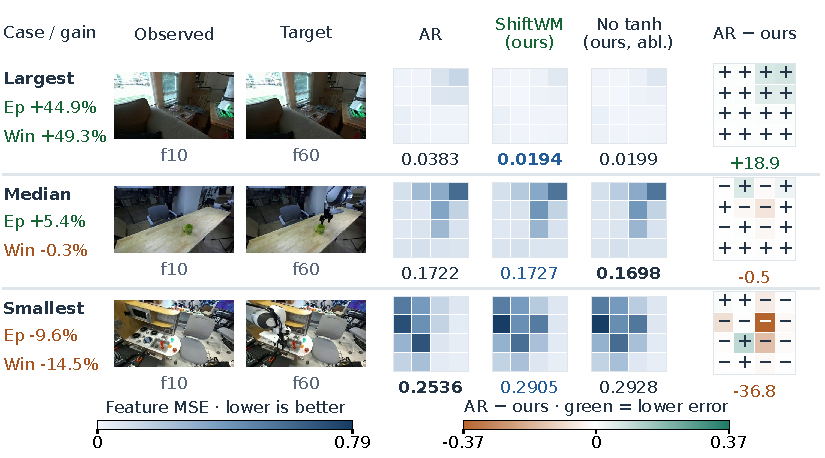
\includegraphics[width=\linewidth]{generated/qualitative_closest_v1/droid_matched.pdf}
\caption{\textbf{Matched forecasts, including the closest component.}
Original largest, median and smallest episode-gain cases from 141 DROID
development episodes, each at its first eligible window. Ep averages all
episode windows; Win describes the shown window. The recorded observation
is the last of three input frames; it and the withheld target are recorded,
not generated images. Three-seed native $h=10$
feature MSE maps share one linear scale across every case and method; bold
scores are the lowest displayed point estimates within a case. The
no-$\tanh$ column is our component ablation. Signed maps subtract ShiftWM's
error from AR's; green/+ means lower error and brown/$-$ higher error.
Signs denote direction, not significance. Numbers
below signed maps are mean differences multiplied by $10^3$. Grids represent
16 semantic feature locations, not pixel-level saliency. Native frame indices
are shown; each forecast step consumes five commands. DROID: CC BY 4.0.}
\label{fig:editorial-qualitative}
\end{figure}
